\section{Conclusions}
The previous chapters of this thesis have presented an effort to build a modeling framework to better understand the propagation and onset of the SCTLD, as well as the impacts of major hurricanes on the transport processes over coral reefs. This model had to be able to accurately capture ocean circulation at different scales to study transport processes in the FRT. First, the large-scale Loop Current-Florida Current system had to be accurately reproduced to correctly capture its impact on eddy formation near the DRTO and the Florida Keys. Second, the model had do resolve ocean circulation at the reef-scale to capture recirculation and acceleration of currents between reefs and islands. This was performed by coupling the multi-scale ocean model SLIM to a connectivity-based epidemiological model (chapter \ref{chap:sctld}), a sediment transport model (chapter \ref{chap:onset}) and a spectral wave model (chapter~\ref{chap:irma}).

The developed coupled hydro-epidemiological model reproduced the observed propagation of the SCTLD through the FRT by modeling the transport of its causative agent within neutrally buoyant material driven by mean barotropic currents. It confirmed the result of previous ex situ studies that showed evidence of waterborne transmission of the SCTLD with an averaged transmission time of the order of 10 days. Furthermore, by using coral resistance to the disease as a parameter, our model results suggested that, on average, corals had pretty low resistance against the disease. This confirmation of experimental results by model results illustrates the important potential of models in evaluating hypotheses derived based field observations on large scale systems. As such, models informed and confronted against field knowledge are a powerful tool to inform the management of complex ecosystems such as a barrier reef.

This epidemiological model was then used to build networks of potential exchanges of disease agents between reefs during a period of three years. The analysis of these networks showed that exchanges from the western end of the DRTO were interrupted during most of 2020. This interruption was likely linked to eddy activity near the DRTO and was consistent with the apparent stalling of the outbreak in the region in 2020. This confirms the role played the Loop Current/Florida Current system in the control of the connectivity in the Florida Keys and the DRTO. Furthermore, location predicted to be more vulnerable to SCTLD in the disease networks were consistent with the observed geographic distribution of disease coral in the DRTO. This further highlights that modeled hydrodynamics are highly explanatory of the propagation of the disease.

The results of chapters \ref{chap:sctld} and \ref{chap:drto} show that the developed high-resolution biophysical is a valuable tool to understand the spread of SCTLD in Florida. The model successfully reproduced the observed propagation of the disease in 2018-2019 and allowed to link the observed stalling of SCTLD to observable hydrodynamic features. Furthermore, the model allowed to deduce potential characteristics of the disease agent and its vector. This highlights the potential of  model to understand the driving mechanics of ongoing outbreaks. Furthermore, indicators such as the vulnerablity and source indicators developed in chaper \ref{chap:drto} could be useful to predict and/or mitigate the spread of SCTLD in other territories of the Caribbean.

Using a sediment transport model, we investigated the impact of the PMDDP on the onset of the SCTLD outbreak in 2014. Our results suggest that the dredging operations had close to no direct impact at Virginia Key monitoring site, identified as the first affected reef. However, reefs affected earlier could have been reached by chopped rock particles produced at the dredged channel. Moreover, our epidemiological model suggested that disease propagation from these reefs to Virginia Key was possible. Sediments released by the PDMMP might therefore have impacted the initiation of one of the worst coral disease outbreaks to date in the Caribbean. These results could have repercussions on the planning of future major dredging projects in the area. FCR is routinely suffering from important anthropogenic stresses caused by the intense activity of the area of Miami. Hence, coastal developments harm coral reefs in two ways: first, by increasing water turbidity and sedimentation during the dredging, and then by causing an increase in pollution and shipping activities. Such adverse impacts should be taken into account when planning dredging operations. The results of chapter \ref{chap:onset} suggest that the potential to initiate a coral disease outbreak should now also be taken into account when considering future dredging project.

Finally, we developed a couple wave-current model to study the impact of Hurricane Irma on transport processes in the Florida Keys. This tropical cyclone was selected because it hit coral reefs during their reproduction period. This coupled modeled correctly reproduced the observed wave and hydrodynamics during the passage of the hurricane. Furthermore, model results suggested that an import dissipation occurred over coral reefs through depth-induced wave-breaking and bottom friction. This important dissipation produced a large wave radiation stress gradients, which caused differences in modeled velocity of up to 1 m/s between the coupled and uncoupled model runs. However, wave-induced transport was dominated by the Stokes drift, which yielded an impact four times larger than the radiation stress gradient. Results of chapter \ref{chap:irma} strongly advocates for the use of coupled wave-currents to accurately model the dispersal of coral larvae under storm conditions. Although we built the tools to study the impact of hurricane on the exchanges of larvae between reefs by developping the coupled SLIM+SWAN, we did not evaluate the impact of Irma on reef connectivity by lack of time.

In conclusion, we answered the four research questions defined in chapter \ref{chap:intro}:

\begin{list}{}{%
    % \setlength{\listparindent}{-0.23in}%
    \setlength{\leftmargin}{0in}%
    % \setlength{\itemindent}{-0.23in} 
    }
    \item \textbf{1. Can we explain the observed spread of SCTLD throughout Florida using an epidemio-hydrodynamic model ?}
    \begin{list}{}{\setlength{\topsep}{0pt}}
        \item Yes, by modeling the transport of disease agents as neutrally buoyant material within the water column, and by calibrating a connectivity-based epidemiological model with field data, we managed to reproduce the observed spread of SCTLD through the FRT. 
    \end{list}
    \item \textbf{2. What caused the apparent stalling of the propagation of SCTLD ?}
    \begin{list}{}{\setlength{\topsep}{0pt}}
        \item Our results suggest that there was an interruption of hydrodynamic-driven exchanges from the Florida Keys to the DRTO during most of 2020, which prevented the propagation of disease agents westward. This interruption of the disease connectivity pathways to the DRTO was likely related to the local eddy activity generated by the meandering of the Florida Current.
    \end{list}
    \item \textbf{3. What was the impact of the PMDDP on the onset of the oubreak of SCTLD~?}
    \begin{list}{}{\setlength{\topsep}{0pt}}
        \item Modeling of sediment transport suggests that the chopped rock particles produced by the dredging activities reached reefs where signs of disease were reported during the first half of 2014. Furthermore, the modeled disease connectivity suggested that disease propagation from these sites to Virginia Key was possible prior to September 2014. The sediments released by the PMDDP might thus have influenced the observed onset of the SCTLD outreak at this site.
    \end{list}
    \item  \textbf{4. What is the effect of hurricane-induced wave-current interactions on transport processes and should they be taken into account when modeling the dispersal of coral larvae ?}
    \begin{list}{}{\setlength{\topsep}{0pt}}
        \item Results of a coupled wave-current model suggest that wave-induced transport under storm conditions dominated by Stokes drift can yield differences in particle trajectories of up to 20 km. Wave-current interactions should thus be taken into to accurately model the dispersal of coral larvae during hurricanes.
    \end{list}
\end{list}


\section{Perspectives for future works}

\subsection*{Combining disease and larval connectivity}
All chapters dedicated to SCTLD rely on the concept of connectivity. In this context, connectivity negatively impacts coral reefs as it yields the propagation of disease agents. Larval connectivity, on the other hand, promotes the resilience of the reef network as it allows the recolonization of depopulated reefs after extreme events such as mass bleaching, hurricanes or disease outbreaks. Larval connectivity is therefore a valuable tool to inform coral reef protection and restoration. Identifying reefs with large out-degree our centrality in the connectivity network indicates the optimal sites for coral outplants in the context of active restoration. Furthermore, knowledge about larval allows to build robust and sustainable networks of connected marine protected areas. Connectivity appears thus to be a double-edged sword. As SLIM allows the computation of larval connectivity \citep{thomas2014numerical,frys2020fine}, a possible application of the tools developed in this thesis is the combination of both types of connectivity.  This combined information would allow to identify reefs that have high potential for restoration and low vulnerability to the disease. A possible measure of the restoration potential is the (weighted) out-degree of reefs in the larval connectivity network, as reefs with strong and numerous outgoing connections in the network are more likely to send many larvae to many connected reefs. Vulnerability to disease can be evaluated using the (weighted) in-degree of reefs in the disease connectivity network, as reefs with strong and numerous incoming connections are more likely to receive more disease agents from many connected reefs. Therefore, reefs with high restoration potential and low vulnerability would correspond to reefs with large larval(weighted) out-degree and low disease (weighted) in-degree. This approach have been applied in \cite{holstein2022} and could be further developed in future studies using more complex connectivity metrics such as the PageRank index \citep{frys2020fine}. 

\subsection*{Improvement of the epidemiological model}
A limitation of the epidemiological model developed in chapter \ref{chap:sctld} is that it uses species-averaged parameters and assumes an uniform distribution of coral reefs throughout the FRT. The fact that our model correctly reproduced the observed spread of SCTLD for a well-defined range of values of coral resistance to the disease highlights the important impact of this parameter on the propagation of the disease. However, coral susceptibility to SCTLD can significantly vary between species and ranges from highly susceptible (\eg~\textit{Dichocoenia stokesii}, \textit{Meandrina meandrites}) to intermediately susceptible (\eg~\textit{Orbicella faveolata}, \textit{Montastrea cavernosa}) and weakly susceptible (\eg~\textit{Acropora Palmata}, \textit{Acropora cervicornis}). A first improvement could therefore be to consider classes corals with different susceptibilities and therefore different infection and removal parameter values in the model. Such improvement would be technically challenging as it would increase the number of variables of model. The development of the model could therefore require the use of more advance graph theory tools such as the multilayer networks \citep{kivela2014multilayer,pilosof2017multilayer}. Furthermore, increasing the number of parameters will thus make their calibration more complex. Moreover, this new modeling framework would require estimates of the distribution of the different coral species across the FRT. Again, compiling this data and deriving realistic estimates would represent a significant challenge. Adding species-specific or location-specific parameters in the model would also allow the evaluate the impact of disease mitigating actions. Lesion treatment using antibiotics could for instance be taken into account in the model by locally reducing the transmission and/or removal parameters. The model parameters could also be made time-dependent as SCTLD progression was reported to slow down during warmer months in the US Virgin Islands \citep{meiling20203d}. Another improvement would be the inclusion of additional processes in the model. For instance, reinfection by SCTLD is currently not possible as corals are "removed" once they are affected by the disease. Given the high mortality of the disease, the "removed" state of the model was assumed equivalent to "dead". However, one might want to discriminate between coral recovery and mortality. However, again, adding processes implies an increase in the number of parameters to be calibrated.

\subsection*{Better understanding the protective role of corals against storm waves}
Simulation results from the coupled wave-current model suggested that storm waves were significantly dissipating over reefs. The modeled significant wave height experiences a twofold reduction over the barrier reef during the passage of the hurricane (Fig. \ref{ccl:swh}). This highlights the important protective role of coral reefs against coastal flood hazard. Better understanding this role can motivate coral reef restoration efforts. For instance, \citep{ferrario2014effectiveness} estimated that coral reefs could provide wave attenuation comparable to artificial defenses such as breakwaters for a lower cost. However, modelling the wave-flow dynamics at the reef scale is particularly challenging and requires models that can explicitly represent small-scale nonhydrostatic processes. The smallest scales that model such as SLIM and SWAN can simulate is limited by the intrinsic assumptions in the model formulations, i.e., hydrostatic for SLIM and phase-averaged for SWAN. These assumptions are no longer valid as soon as the horizontal scales of motion become comparable to the vertical scales \citep{marshall1997hydrostatic}. For such situations, it becomes necessary to couple the SLIM+SWAN model with a phase-resolving nonhydrostatic wave-flow model, hence achieving a multi-physics modelling framework. Nonhydrostatic models are more expensive to run as they require a much finer spatial resolution (~1 m) and have a more complex physics. They can therefore often be used only in rather small areas and over short periods of time \citep{fringer2019future}. One promising approach to tackle this issue would be to use machine learning algorithms to locally emulate the dynamics of a complex high-resolution model and hence speed up the computational process \citep{kasim2021building}. Machine learning is based on the principle of extracting information from data, which can either be observational data or high-resolution model outputs, and deriving relationships between datasets without the need for physics-based models. This procedure has recently been applied to ocean modelling and was able to reproduce the temporal and spatial variability of unresolved turbulent processes, when given a smoothed view of the dynamics \citep{bolton2019applications}. 

\begin{figure}
    \centering
    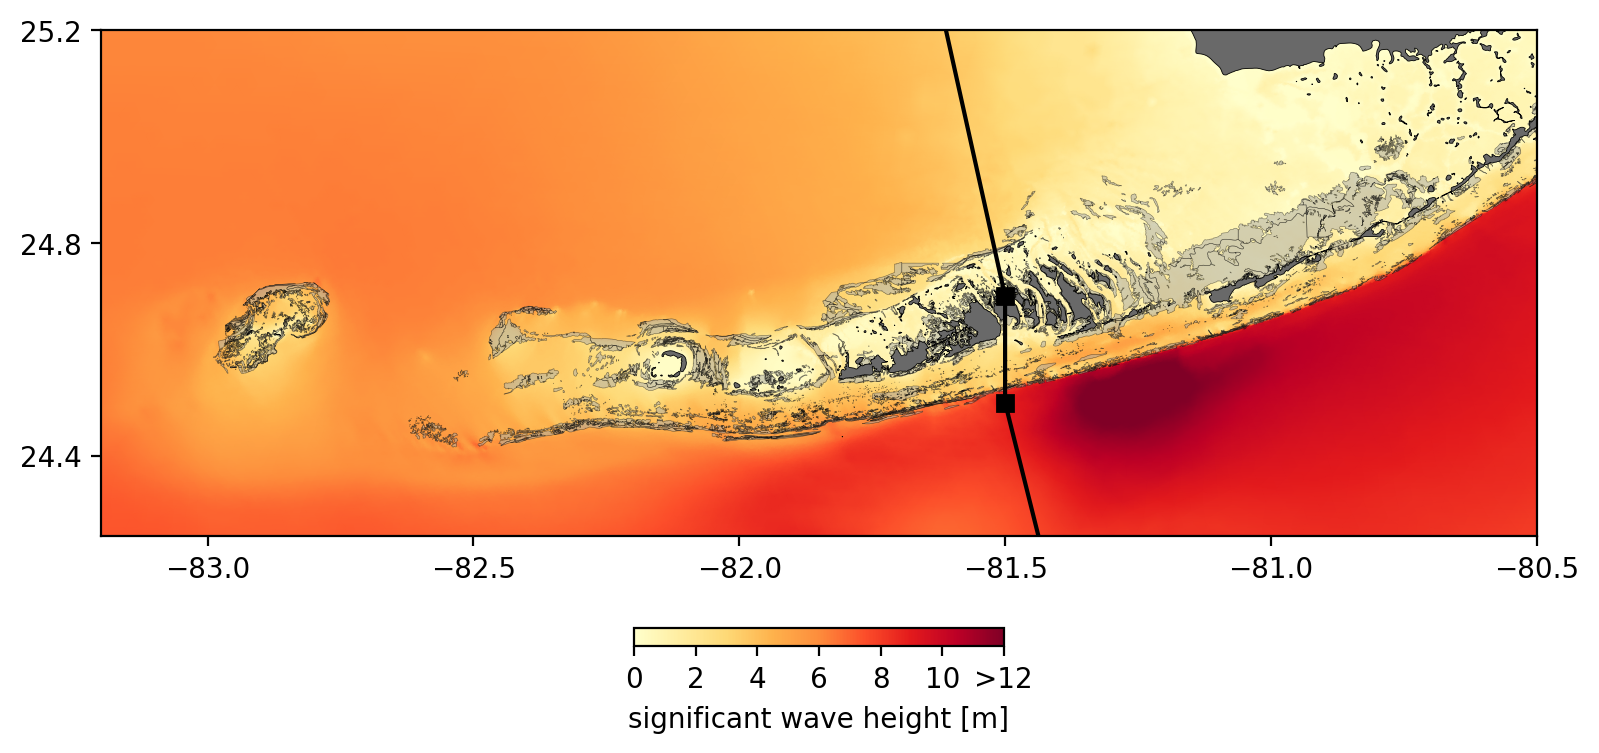
\includegraphics[width=\textwidth]{chapters/conclusions/figures/swh_figure.png}
    \caption{Snapshot of the significant wave height modeled by the coupled SLIM+SWAN model during Hurricane Irma, on Sept 10, 2017 at 1200 UTC. The path of the hurricane is shown by a black line with squares. Land is shown in dark gray and reefs in light gray. Significant wave attenuation is visible between the fringing coral reefs and the islands.}
    \label{ccl:swh}
\end{figure}